\documentclass[a4paper,10pt]{article}
\usepackage[utf8]{inputenc}
\usepackage{graphicx}
\usepackage{float}
\usepackage{url}
\usepackage{hyperref}

\hypersetup{
    colorlinks,
    citecolor=blue,
    filecolor=blue,
    linkcolor=blue,
    urlcolor=blue
}

%Python stuff:
% Default fixed font does not support bold face
\DeclareFixedFont{\ttb}{T1}{txtt}{bx}{n}{12} % for bold
\DeclareFixedFont{\ttm}{T1}{txtt}{m}{n}{12}  % for normal

% Custom colors
\usepackage{color}
\definecolor{deepblue}{rgb}{0,0,0.5}
\definecolor{deepred}{rgb}{0.6,0,0}
\definecolor{deepgreen}{rgb}{0,0.5,0}

\usepackage{listings}

% Python style for highlighting
\newcommand\pythonstyle{\lstset{
language=Python,
basicstyle=\ttm,
otherkeywords={self},             % Add keywords here
keywordstyle=\ttb\color{deepblue},
emph={MyClass,__init__},          % Custom highlighting
emphstyle=\ttb\color{deepred},    % Custom highlighting style
stringstyle=\color{deepgreen},
frame=tb,                         % Any extra options here
showstringspaces=false            % 
}}


% Python environment
\lstnewenvironment{python}[1][]
{
\pythonstyle
\lstset{#1}
}
{}

% Python for external files
\newcommand\pythonexternal[2][]{{
\pythonstyle
\lstinputlisting[#1]{#2}}}

% Python for inline
\newcommand\pythoninline[1]{{\pythonstyle\lstinline!#1!}}

%opening
\title{Plotting with Analysator's MayaVi interface}
\author{Otto Hannuksela}

\begin{document}

\maketitle

\tableofcontents

\newpage

\section{Plotting the grid}

\begin{python}
import pytools as pt
f = pt.vlsvfile.VlsvReader('bulk.0000872.vlsv')
grid = pt.grid.MayaviGrid(f, 'rho')
\end{python}

\section{How to navigate}

In order to navigate, use the mouse scroll to zoom, mouse3 to move the image and mouse 1 to tilt the 
grid.

\section{Picker options}

Analysator has implemented many picker options. These include:

\begin{enumerate}
 \item None
 \item Velocity\_space
 \item Velocity\_space\_nearest\_cellid
 \item Velocity\_space\_iso\_surface
 \item Velocity\_space\_nearest\_cellid\_iso\_surface
 \item Pitch\_angle
 \item Gyrophase\_angle
 \item Cut\_through (See Section \ref{ssec:cutthrough})
\end{enumerate}

\newpage

\subsection{Cut\_through} \label{ssec:cutthrough}

The cut-through option requires specifying the variable to be plotted with the \emph{Args} field in 
MayaVi and needs two clicks somewhere in the MayaVi plot (starting and ending point for the cut-through). 
The cut-through feature is best illustrated in Figures \ref{fig:cut_through1}-\ref{fig:cut_through4}.


\begin{figure}[H]
 \centering
 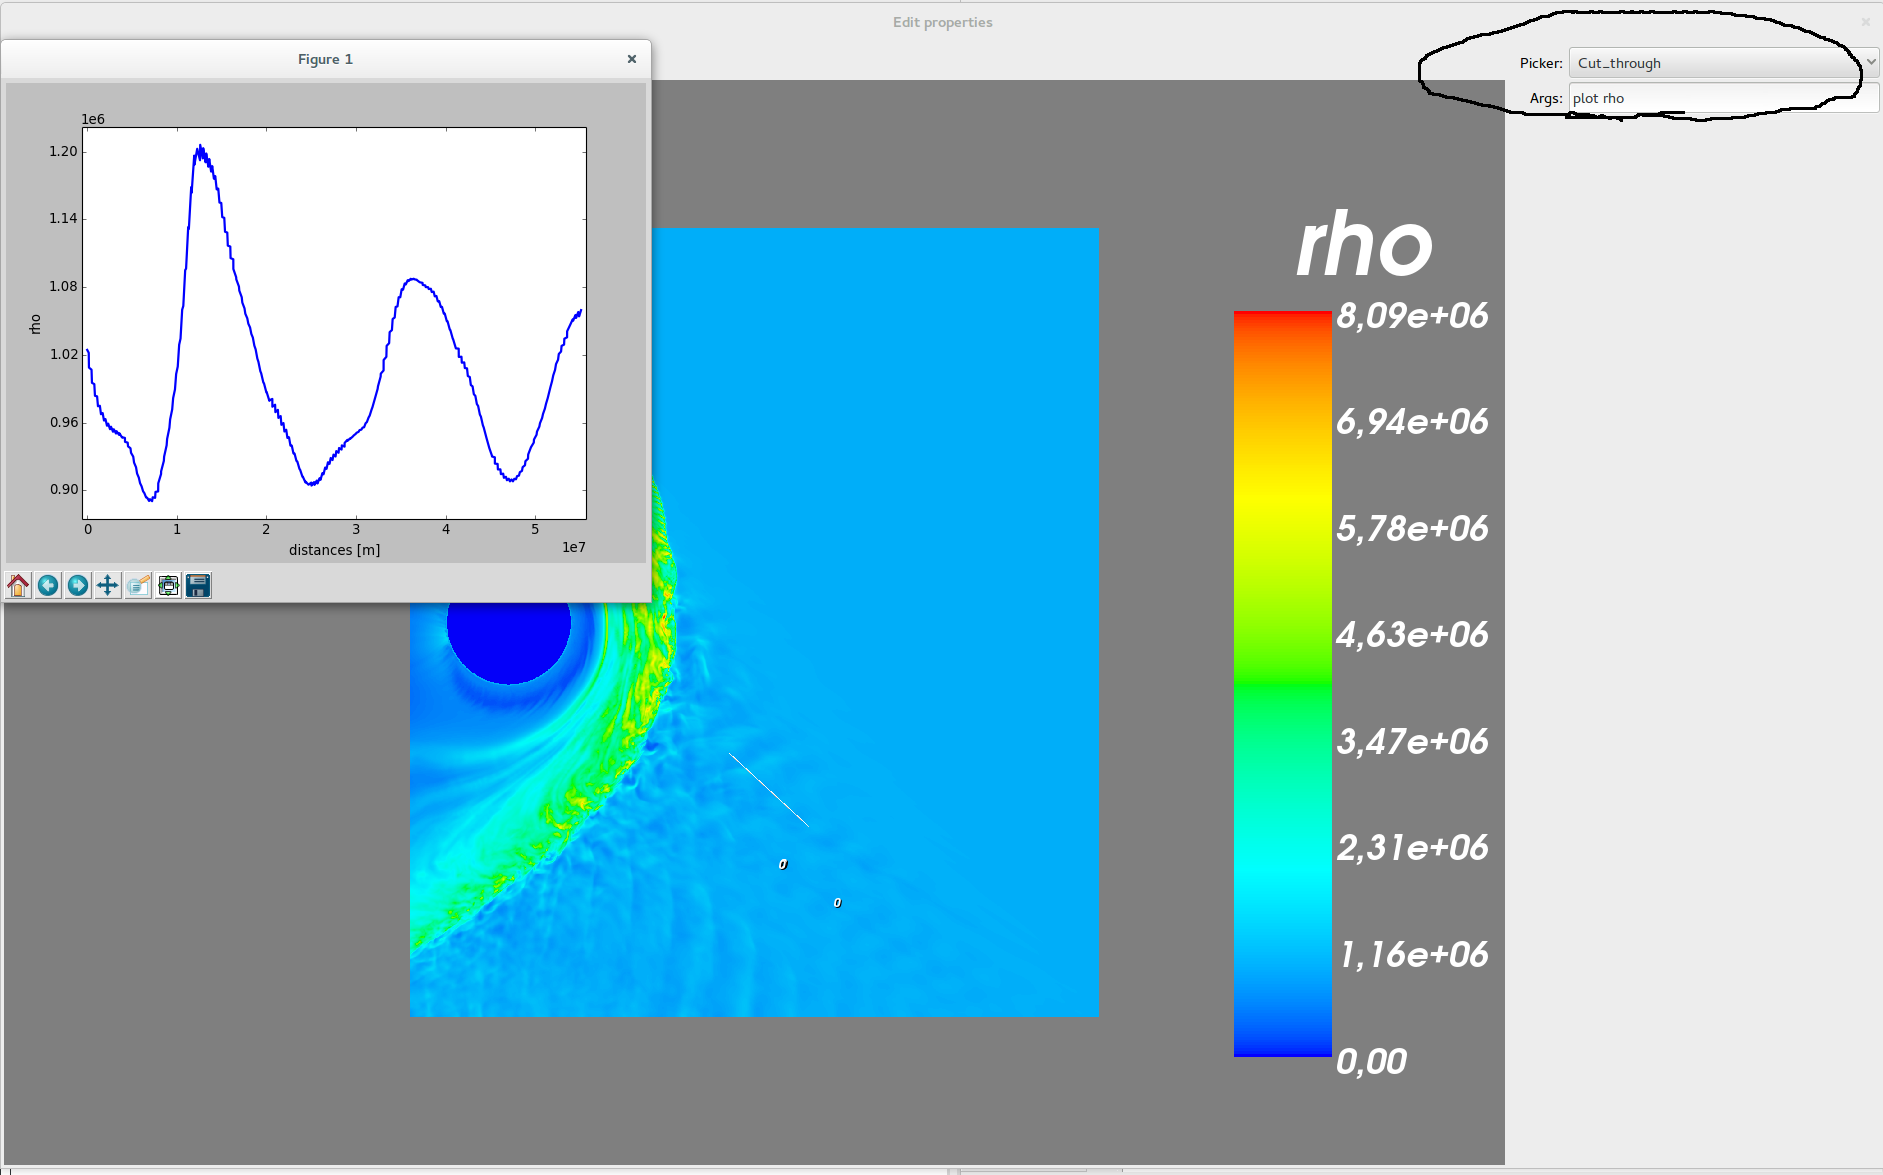
\includegraphics[width=\textwidth]{../../images/cut_through1.png}
 \caption{Example plot with the cut-through function demonstrating its use. The cut-through is drawn as a 
 line and we are plotting the cut-through of rho, as specified in the \emph{Args}-field seen in the picture.}
 \label{fig:cut_through1}
\end{figure}

\begin{figure}[H]
 \centering
 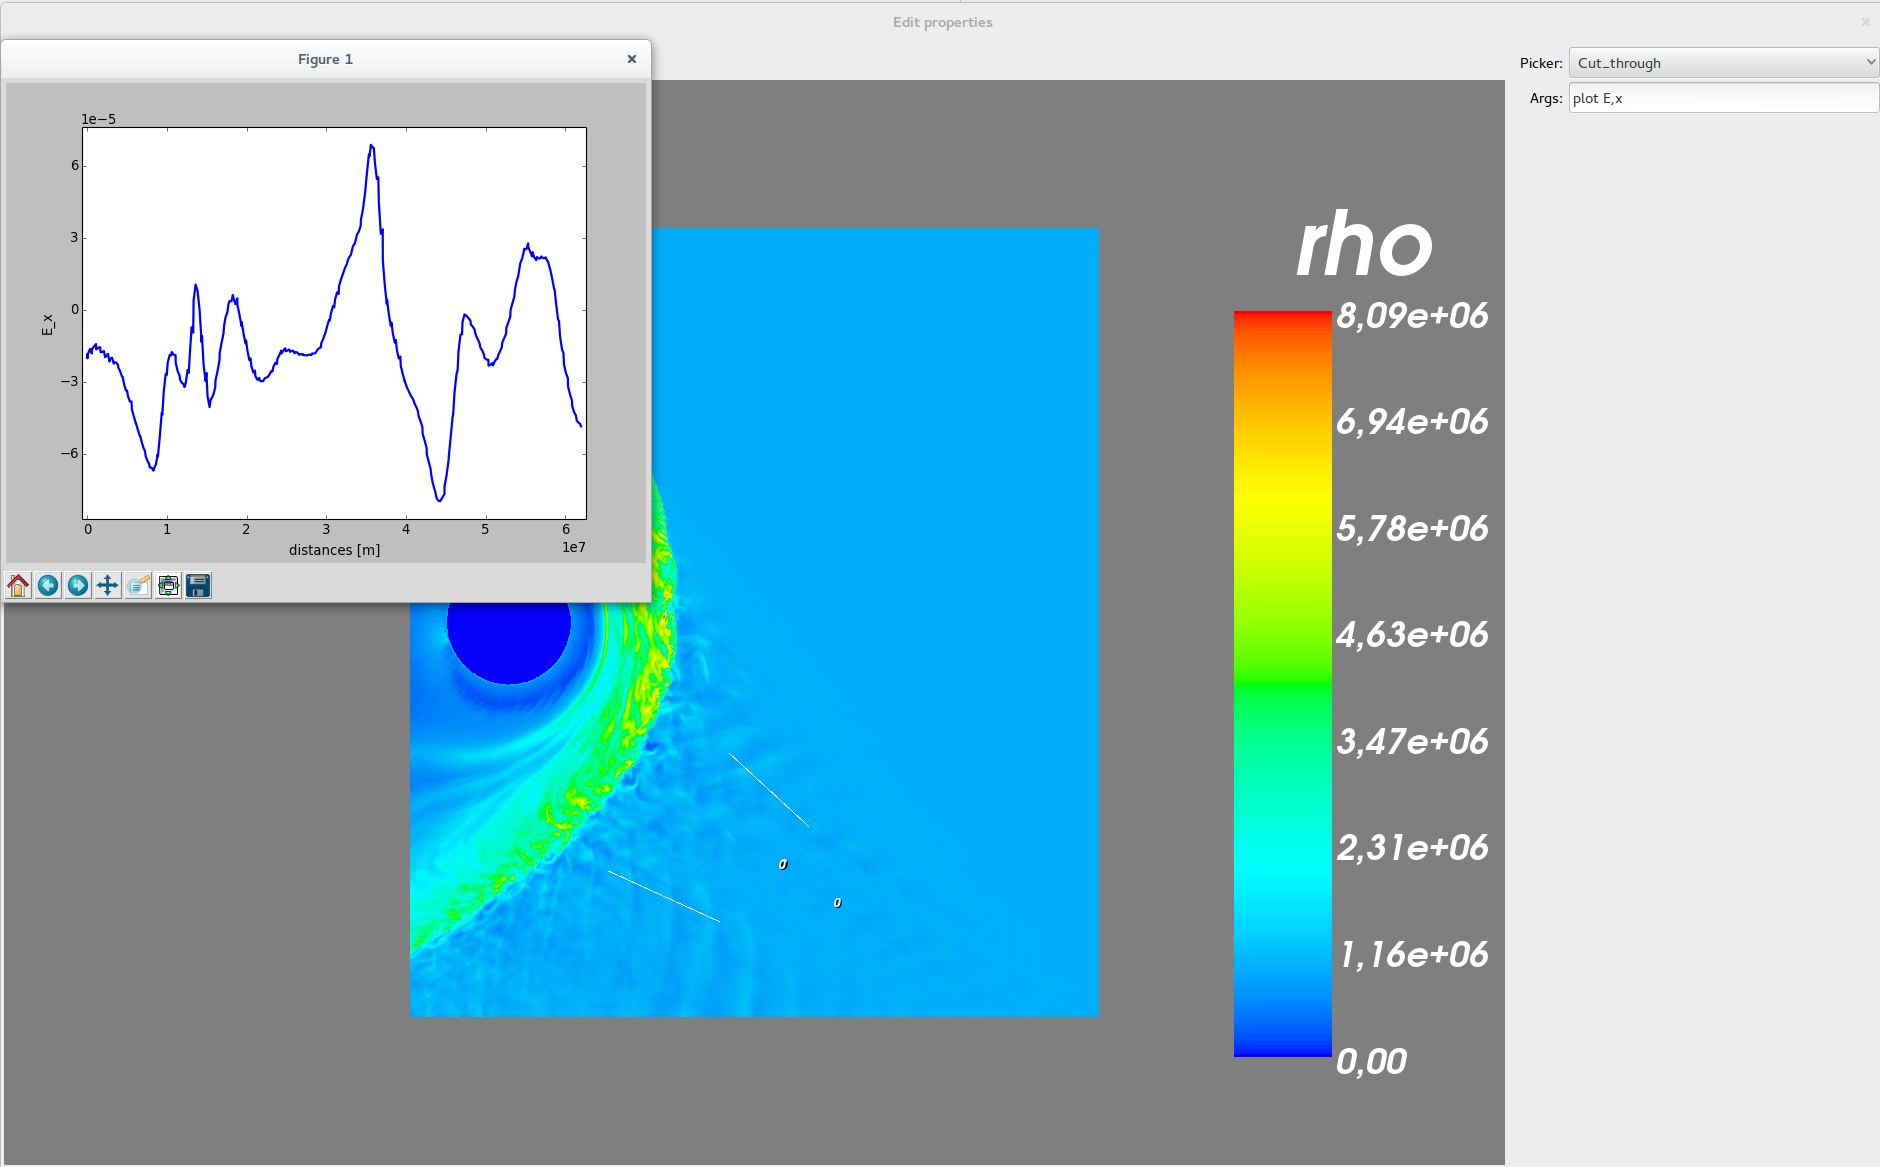
\includegraphics[width=\textwidth]{../../images/cut_through2.png}
 \caption{Example plot with the cut-through function demonstrating its use.}
 \label{fig:cut_through2}
\end{figure}

\begin{figure}[H]
 \centering
 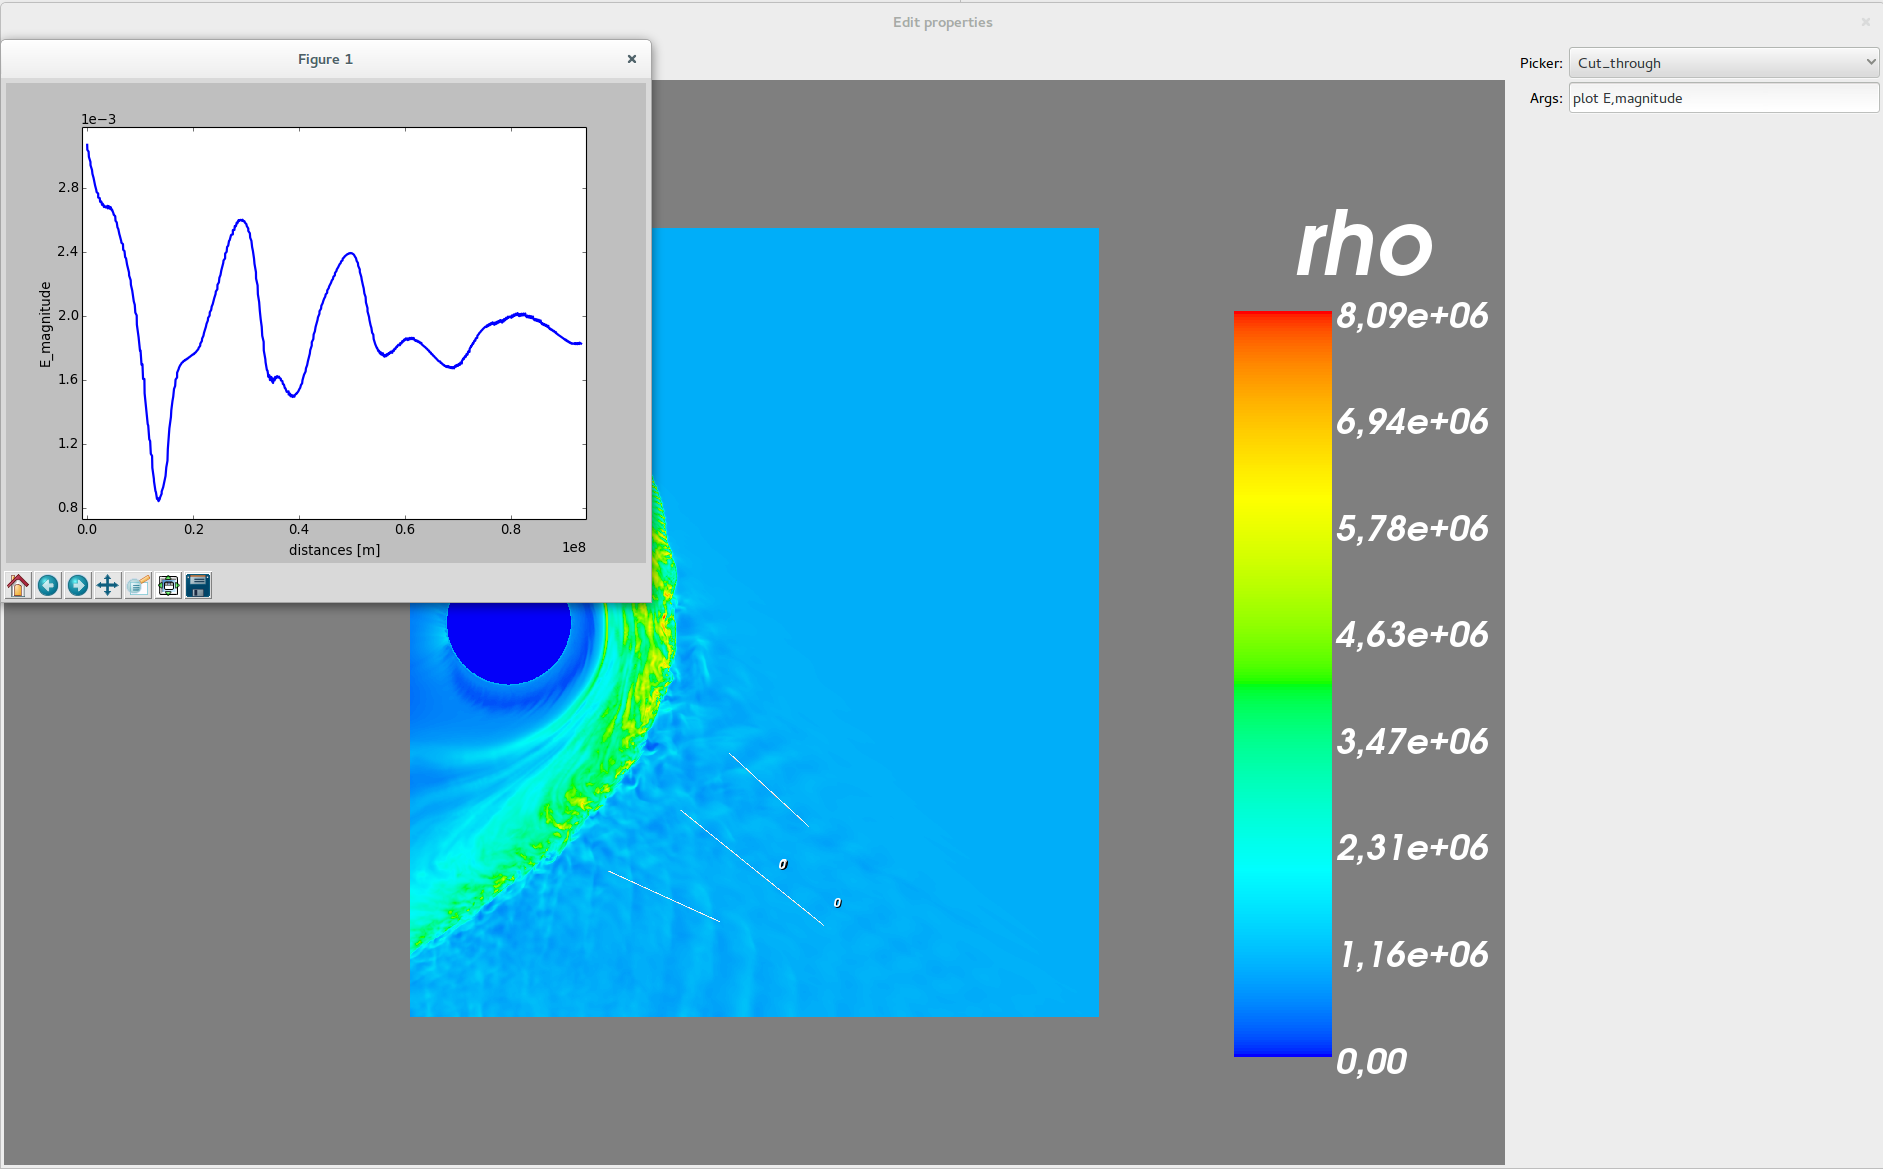
\includegraphics[width=\textwidth]{../../images/cut_through3.png}
 \caption{Example plot with the cut-through function demonstrating its use.}
 \label{fig:cut_through3}
\end{figure}

\begin{figure}[H]
 \centering
 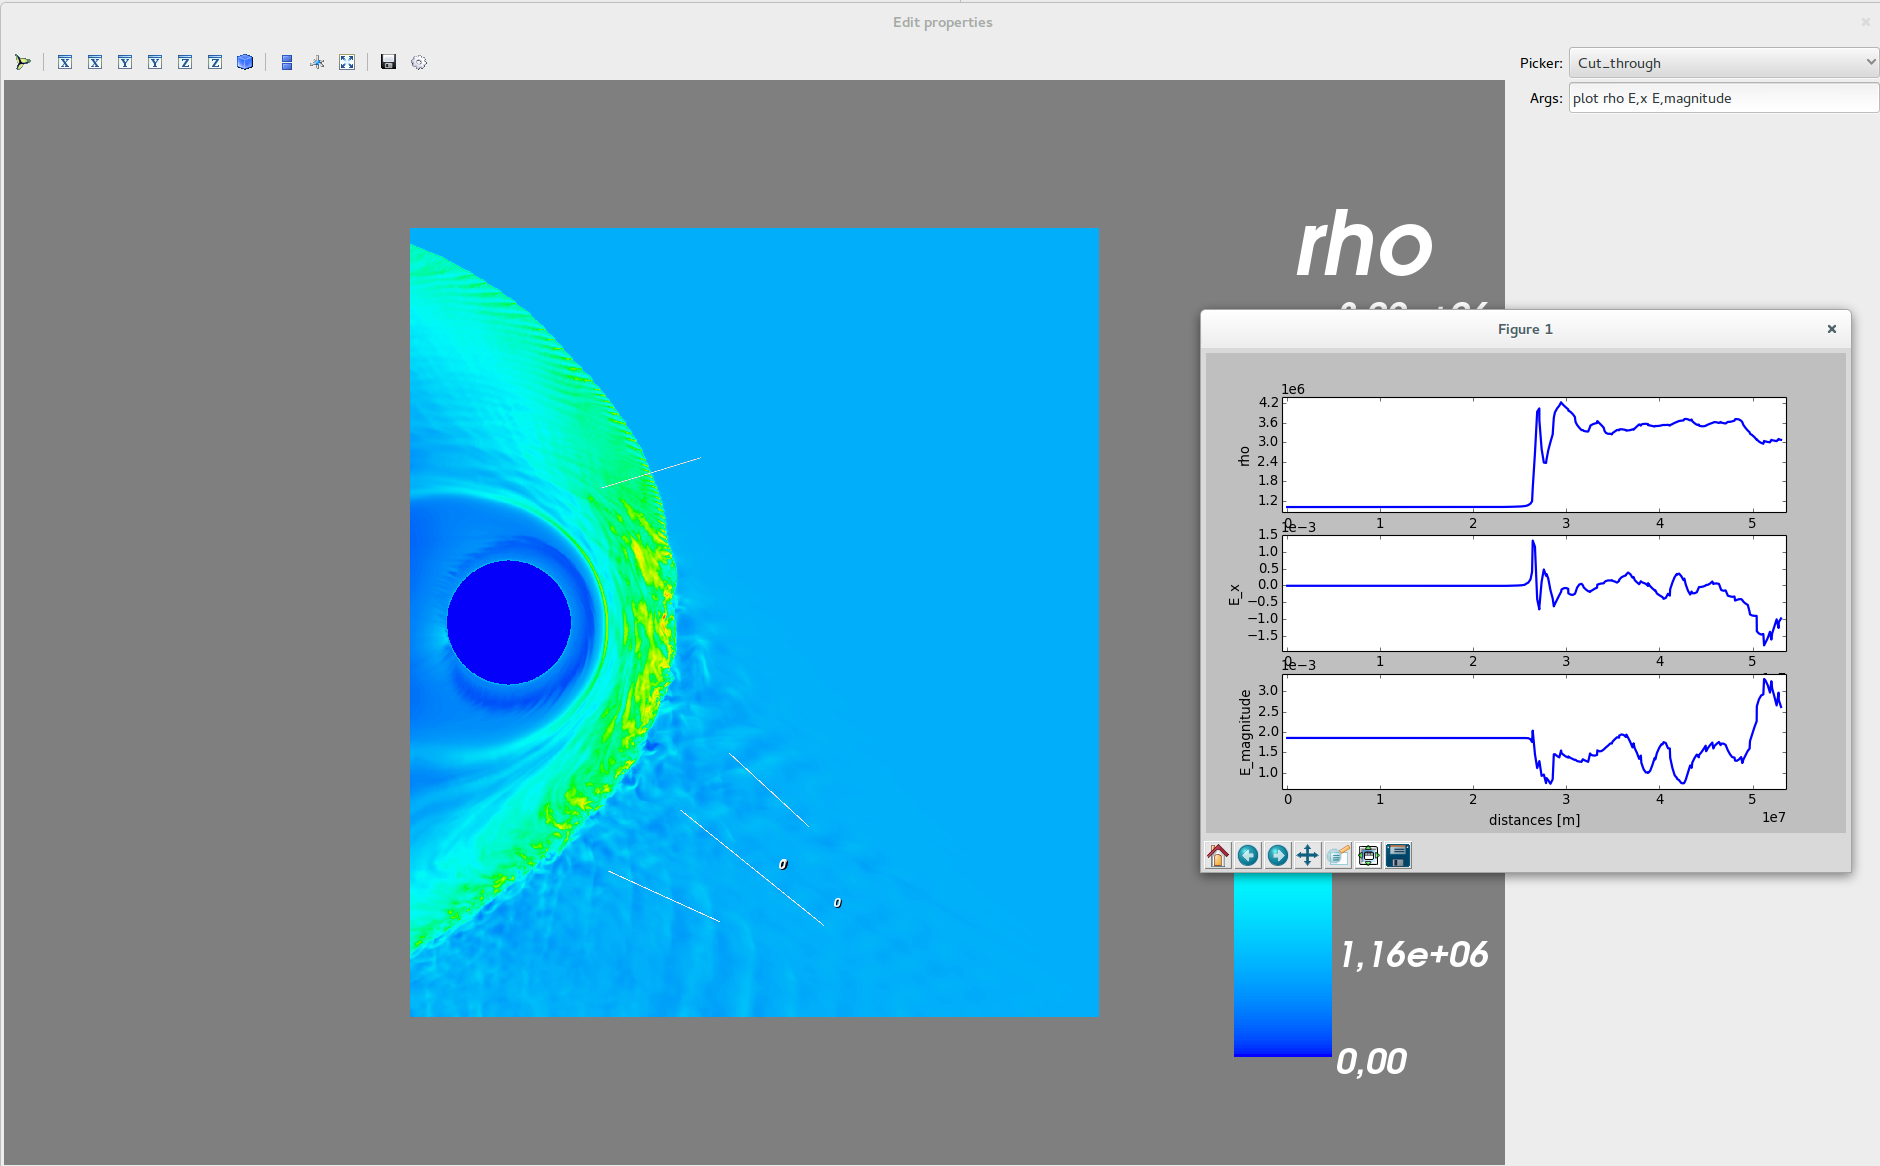
\includegraphics[width=\textwidth]{../../images/cut_through4.png}
 \caption{Example plot with the cut-through function demonstrating its use.}
 \label{fig:cut_through4}
\end{figure}

\newpage

\subsubsection{Cut-through: Example \emph{Args} fields}

Example Args fields:

Plots $rho$:
\begin{python}
plot rho
\end{python}
Plots the x-component of $\mathbf{E}$:
\begin{python}
plot E,x
\end{python}
Plots the magnitude of $\mathbf{B}$:
\begin{python}
plot E,magnitude
\end{python}

\newpage

\subsection{Velocity\_space and Velocity\_space\_nearest\_cellid}

Draws the velocity space for the cell we click on. If there exists no velocity space data in the vlsv 
file for the given cellid, then using \emph{Velocity\_space\_nearest\_cellid} is adviced, as it picks the 
nearest cellid with velocity distribution data and draws it.

Example is shown in Figure \ref{fig:vel_space}

\begin{figure}[H]
 \centering
 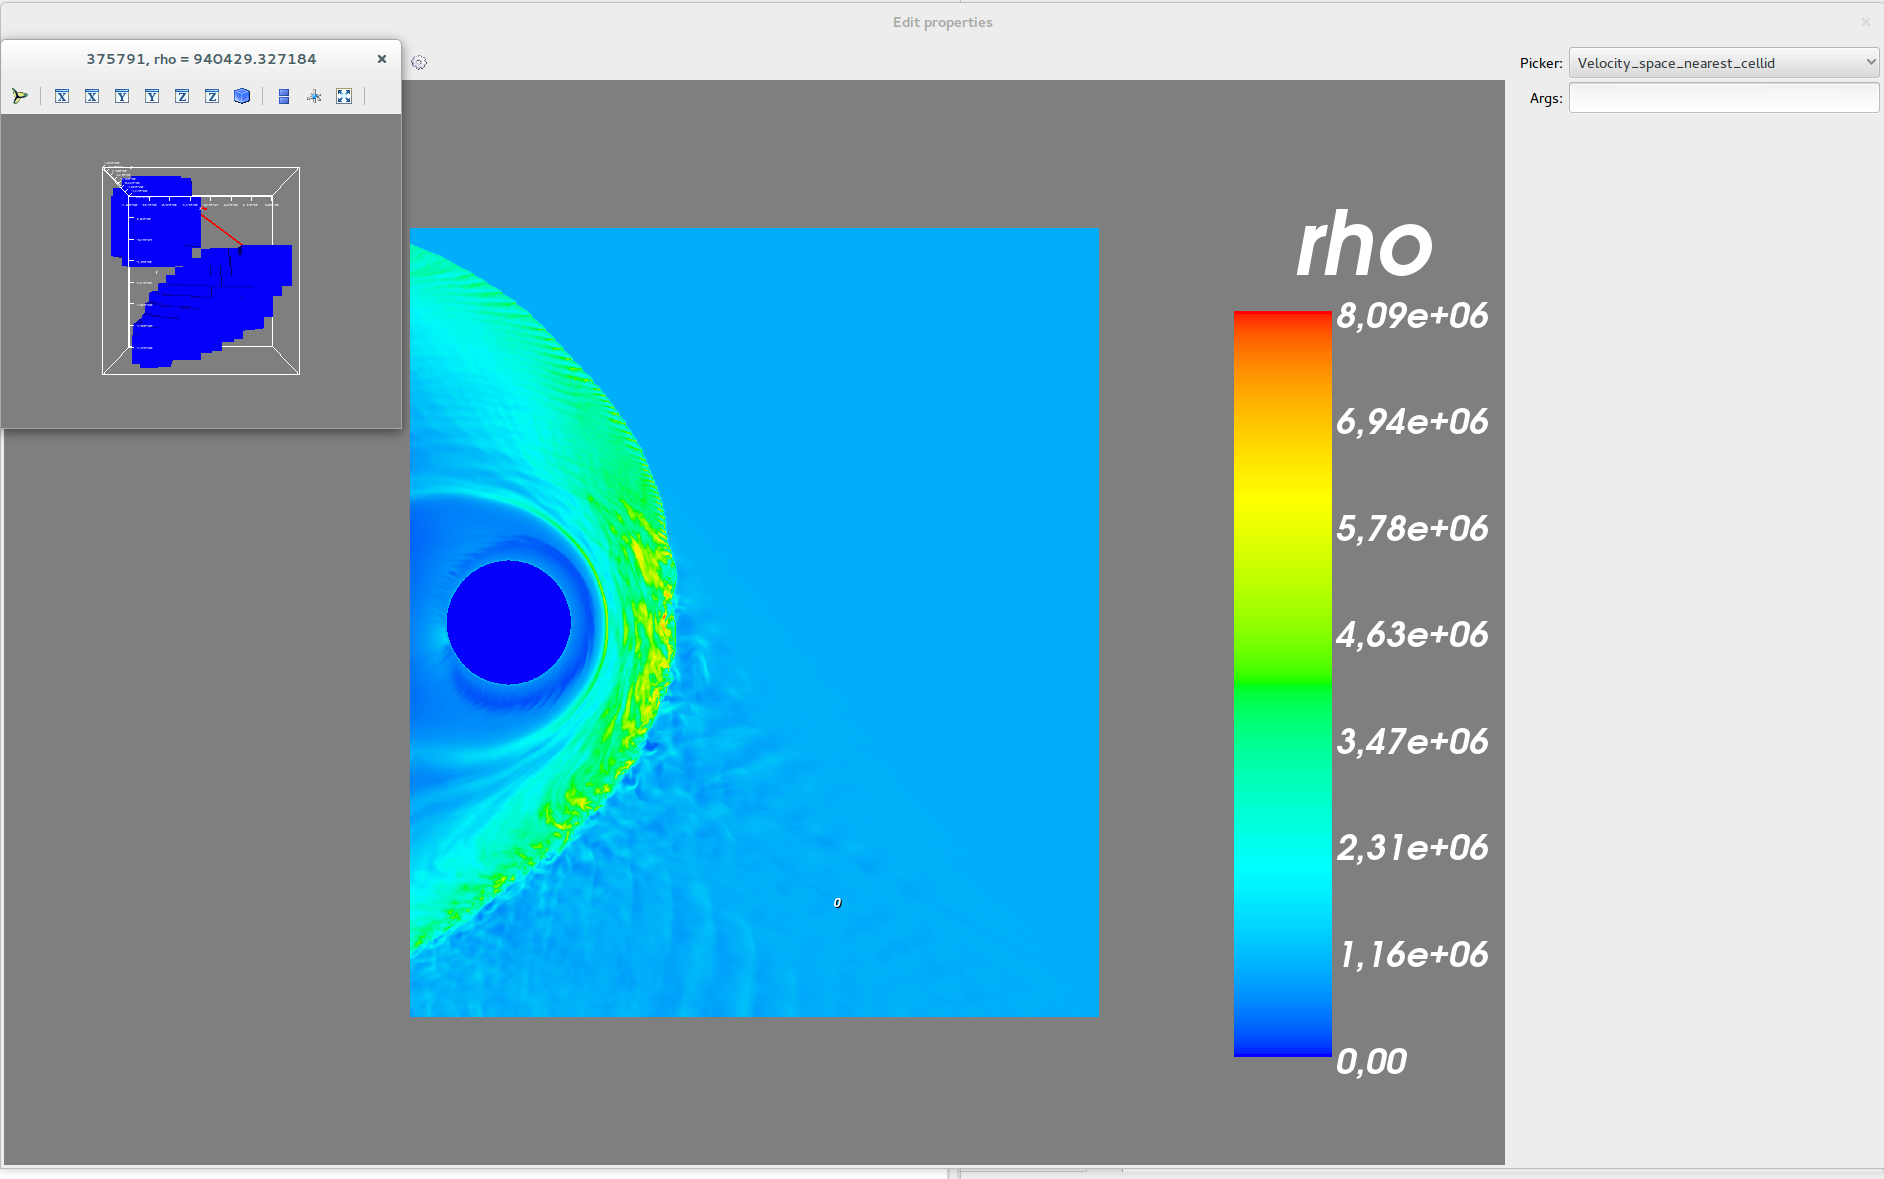
\includegraphics[width=\textwidth]{../../images/velocity_space_nearest_cellid.png}
 \caption{A velocity space drawn for a clicked cellid. The cell is marked with a \emph{0} in the plot.}
 \label{fig:vel_space}
\end{figure}


\subsection{Velocity\_space\_iso\_surface and Velocity\_space\_nearest\_cellid\_iso\_surface}

Same as with Velocity\_space but draws an iso-surface plot.

Example is shown in Figure \ref{fig:vel_space2}

\begin{figure}[H]
 \centering
 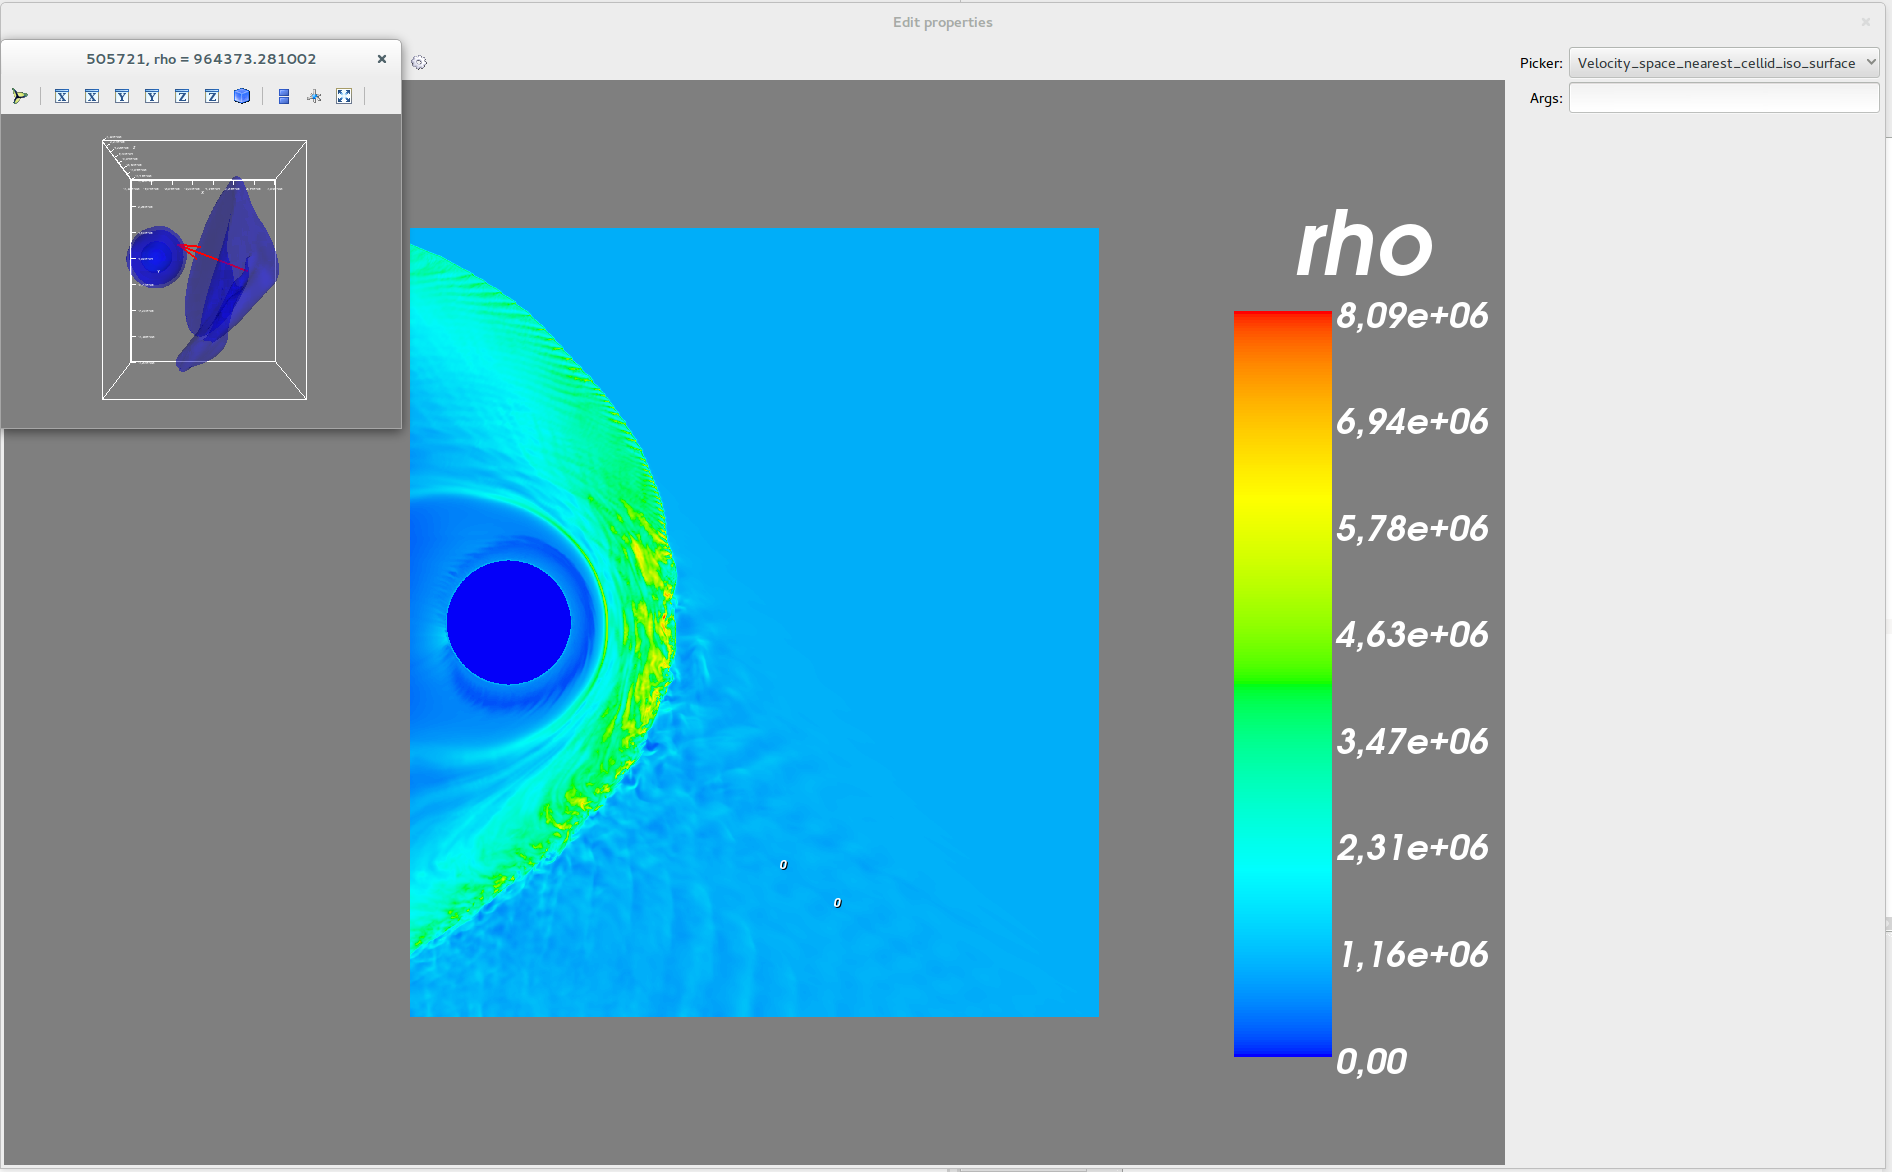
\includegraphics[width=\textwidth]{../../images/velocity_space_nearest_cellid_iso_surface.png}
 \caption{A velocity space drawn for a clicked cellid. The cell is marked with a \emph{0} in the plot.}
 \label{fig:vel_space2}
\end{figure}

\subsection{Pitch\_angle}

Draws a pitch angle plot for a given cell id.

Example: Figure \ref{fig:pitch_angle}

\begin{figure}[H]
 \centering
 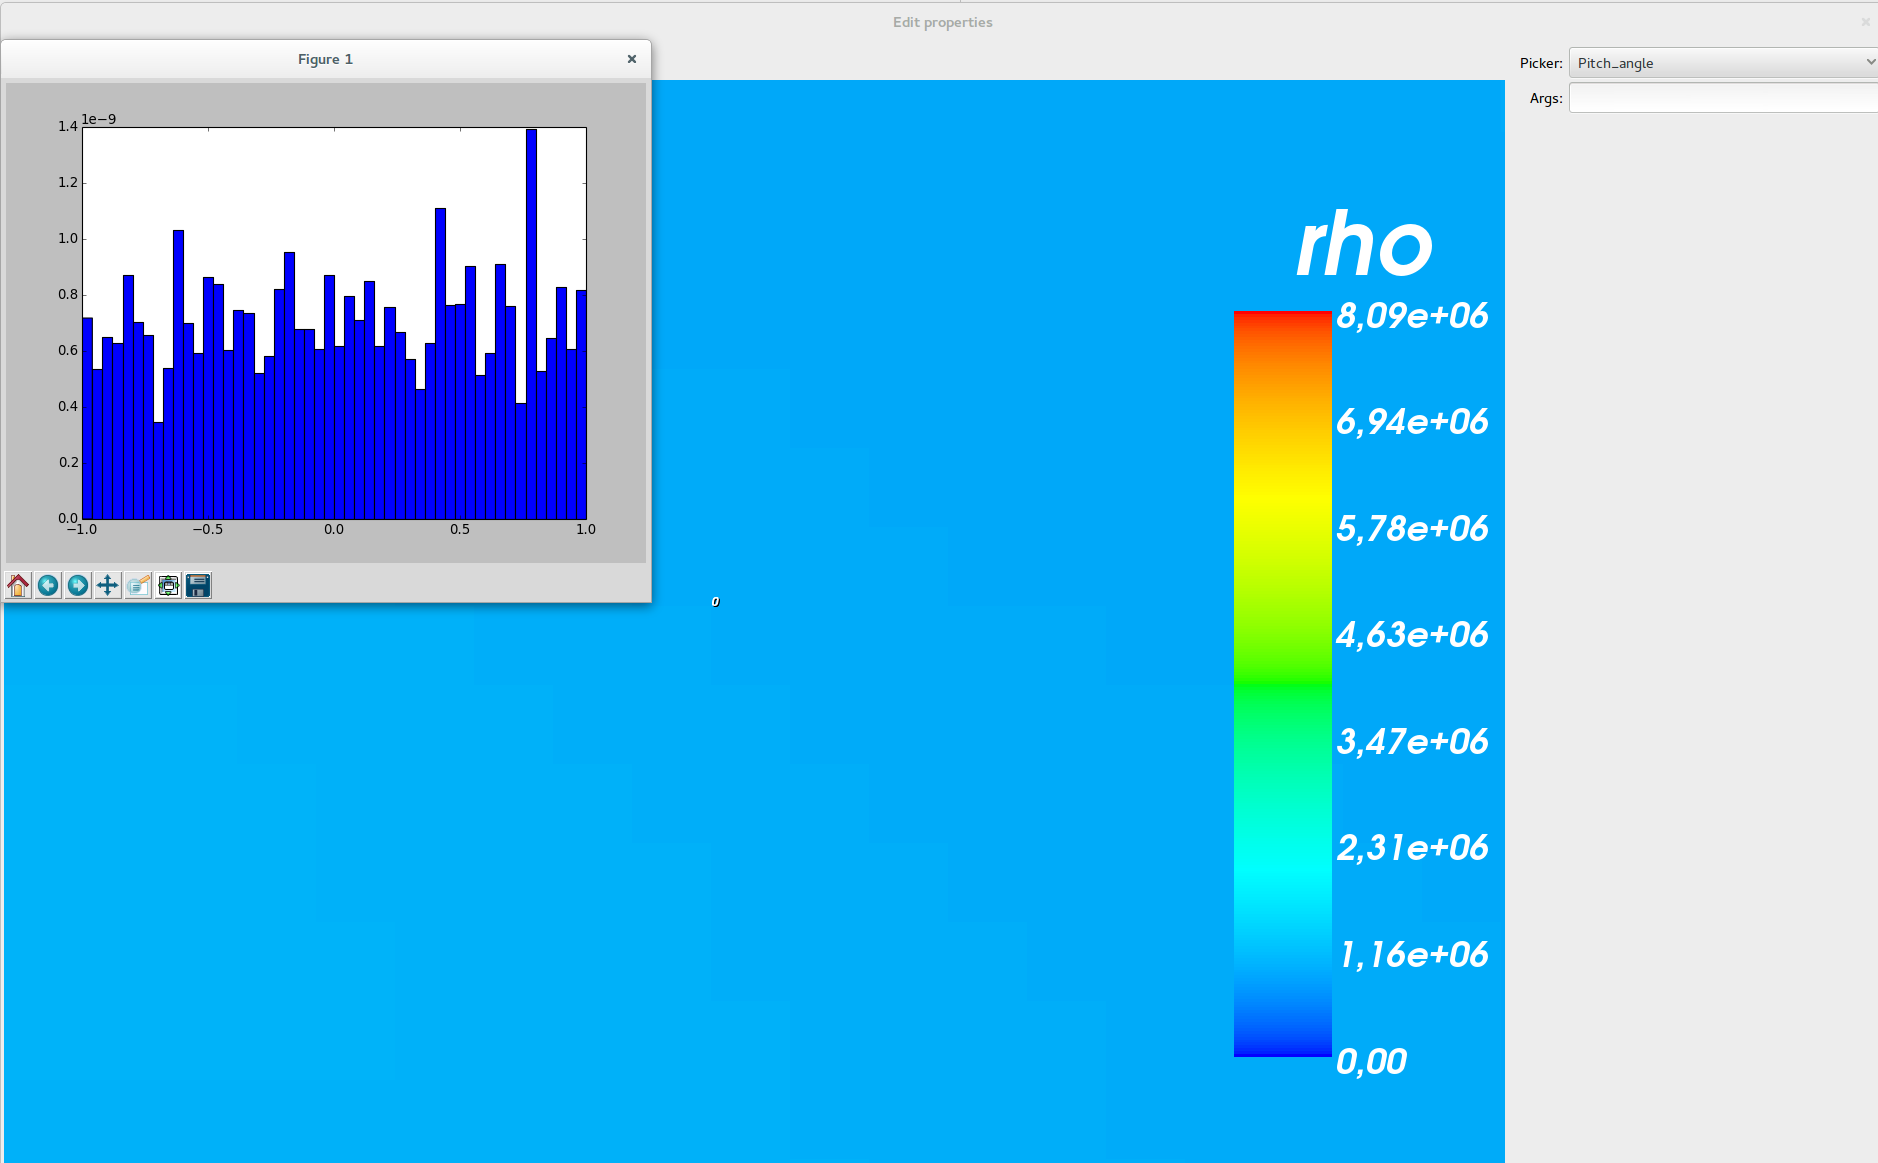
\includegraphics[width=\textwidth]{../../images/pitch_angle.png}
 \caption{A pitch angle plot drawn for a clicked cellid. The cell is marked with a \emph{0} in the plot.}
 \label{fig:pitch_angle}
\end{figure}

\subsection{Gyrophase angle}

Draws a gyrophase angle plot for a given cell id. This feature was added to Analysator thanks to Yann's 
contribution.

Example: Figure \ref{fig:gyrophase_angle}

\begin{figure}[H]
 \centering
 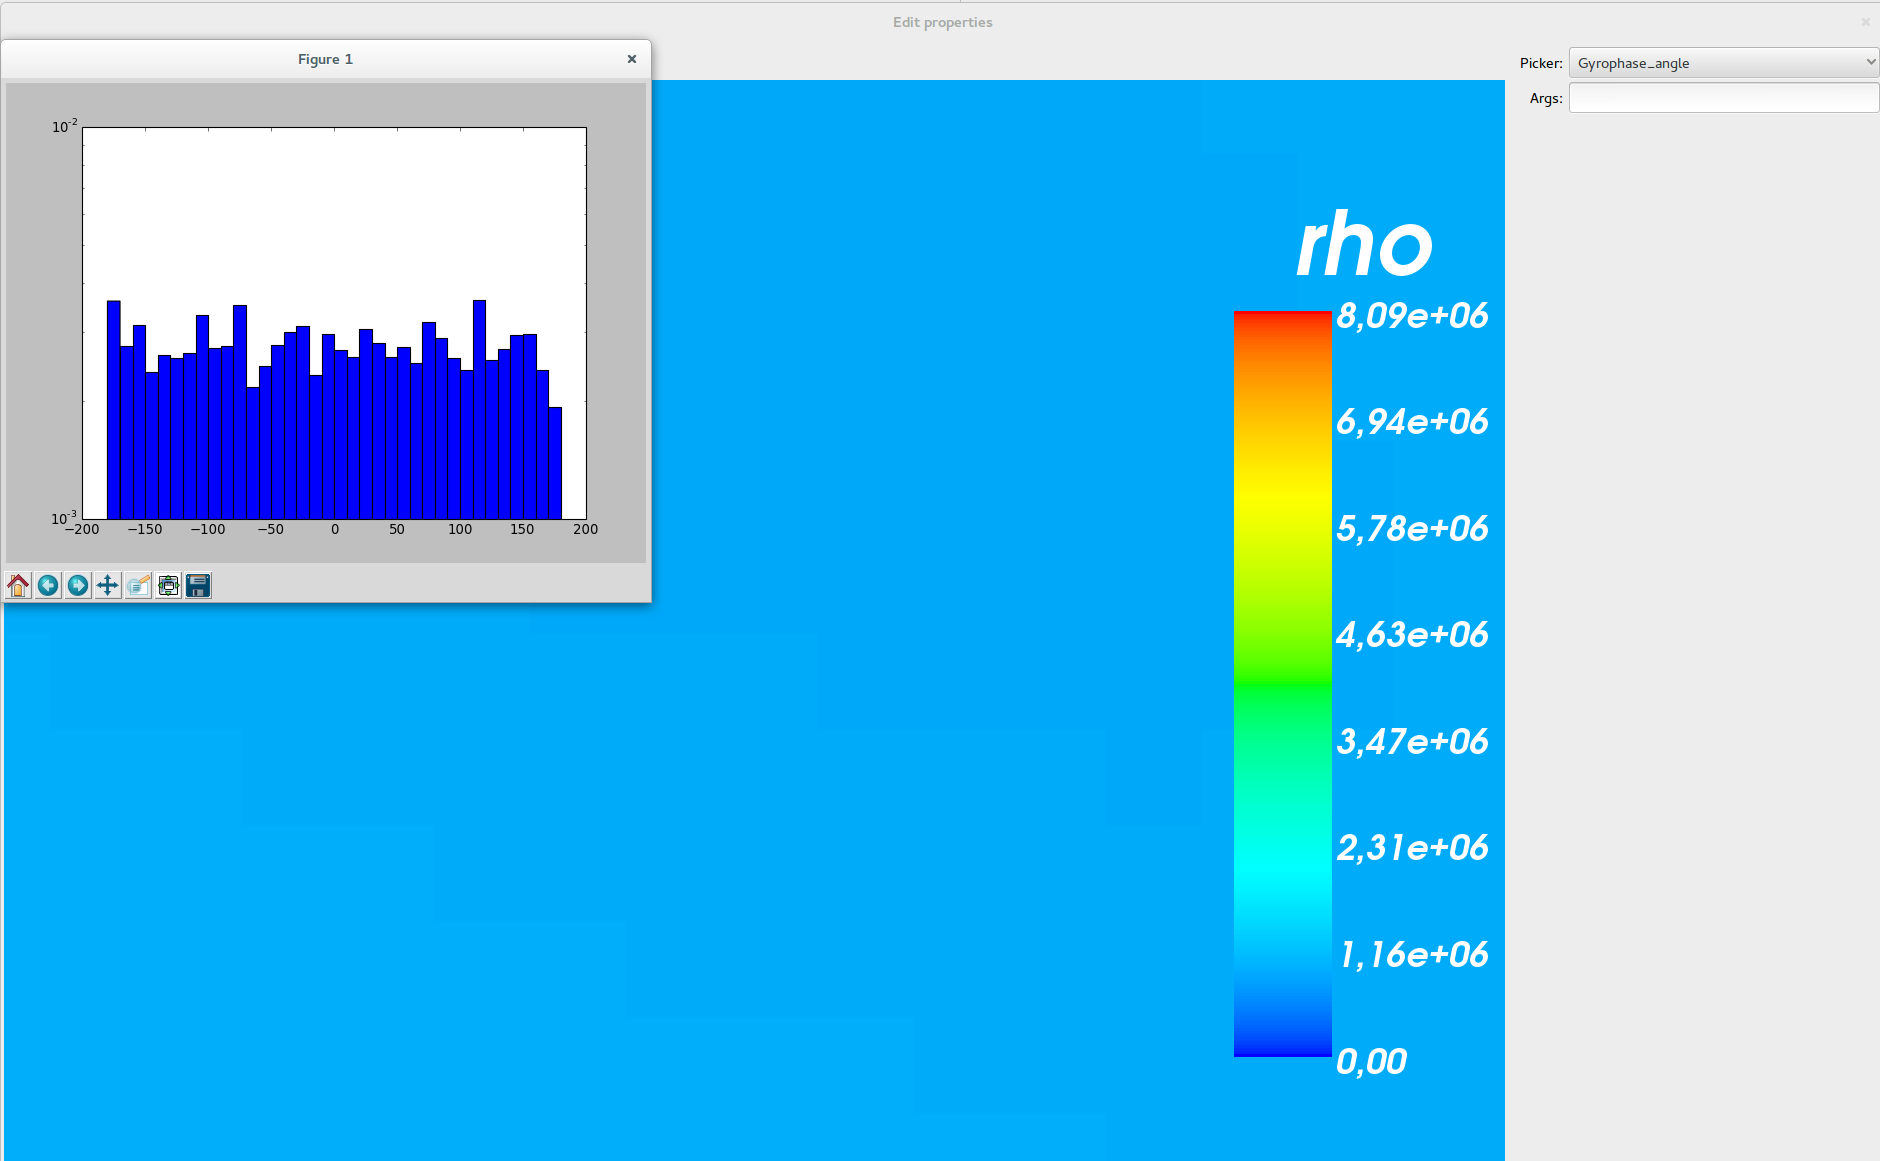
\includegraphics[width=\textwidth]{../../images/gyrophase_angle.png}
 \caption{A gyrophase angle plot drawn for a clicked cellid. The cell is marked with a \emph{0} in the plot.}
 \label{fig:gyrophase_angle}
\end{figure}



\end{document}
